\documentclass[12pt]{article}
\usepackage[utf8]{inputenc}
\usepackage{float}


\usepackage[hmargin=3cm,vmargin=6.0cm]{geometry}
%\topmargin=0cm
\topmargin=-2cm
\addtolength{\textheight}{6.5cm}
\addtolength{\textwidth}{2.0cm}
%\setlength{\leftmargin}{-5cm}
\setlength{\oddsidemargin}{0.0cm}
\setlength{\evensidemargin}{0.0cm}

%misc libraries goes here
\usepackage{amsmath}
\usepackage{fancyvrb}
\usepackage{graphicx}

\begin{document}

\section*{Student Information } 
%Write your full name and id number between the colon and newline
%Put one empty space character after colon and before newline
Full Name : Batuhan Akçan  \\
Id Number : 2580181 \\

% Write your answers below the section tags
\section*{Answer 1}

\subsection*{a)}
We know that $f_{T_A}(t_A) = f_{T_B}(t_B) = \frac{1}{b-a} = \frac{1}{100-0} = \frac{1}{100}$\\
Since $T_A$ and $T_B$ are independent, $f_{T_A,T_B}(t_A, t_B) = f_{T_A}(t_A)\cdot f_{T_B}(t_B) = \frac{1}{100-0} \cdot \frac{1}{100-0} = \frac{1}{10000}$\\
$F_{T_A}(t_A) = \int_{0}^{t_A} \frac{1}{100} dx = \frac{t_A}{100}$\\
$F_{T_B}(t_B) = \int_{0}^{t_B} \frac{1}{100} dx = \frac{t_B}{100}$\\
Since $T_A$ and $T_B$ are independent, $F_{T_A,T_B}(t_A, t_B) = F_{T_A}(t_A)\cdot F_{T_B}(t_B) = \frac{t_A\cdot t_B}{10000}$
\subsection*{b)} 
$P\{T_A < 30\}\cdot P\{40 < T_B < 60\} = F_{T_A}(30) \cdot (F_{T_B}(60)-F_{T_B}(40)) = \frac{30}{100} \cdot (\frac{60}{100} - \frac{40}{100}) = \frac{6}{100} = 0.06$
\subsection*{c)} 
$ \int_{0}^{90} \int_{t_B}^{t_B+10} f_{T_A,T_B}(t_A,t_B) dt_Adt_B + \int_{90}^{100} \int_{t_B}^{100} f_{T_A,T_B}(t_A,t_B) dt_Adt_B =\vspace{0.2cm}\\
\int_{0}^{90} \int_{t_B}^{t_B+10} \frac{1}{10000} dt_Adt_B + \int_{90}^{100} \int_{t_B}^{100} \frac{1}{10000} dt_Adt_B = \int_{0}^{90} \frac{1}{1000} dt_B + \int_{90}^{100} \frac{100-t_B}{10000} dt_B = 0.09+0.1-0.095 \vspace{0.2cm}\\
= 0.095 $
\subsection*{d)} 
$ \int_{0}^{20} \int_{0}^{t_B+20} \frac{1}{10000} dt_Adt_B + \int_{20}^{80} \int_{t_B-20}^{t_B+20} \frac{1}{10000} dt_Adt_B + \int_{80}^{100} \int_{t_B-20}^{100} \frac{1}{10000} dt_Adt_B =\vspace{0.2cm}\\
\int_{0}^{20} \frac{t_B+20}{10000} dt_B + \int_{20}^{80} \frac{4}{1000} dt_B + \int_{80}^{100} \frac{120-t_B}{10000} dt_B = \frac{2}{100} + \frac{4}{100} + \frac{24}{100} + \frac{24}{100} - \frac{18}{100} = 0.36  $

\section*{Answer 2}

\subsection*{a)} 
$65\%$ of 150 is approximately 98 customers. Probability of being a frequent shopper is 0.6, not being a frequent shopper is 0.4. At least 98, at most 150 customers can be frequent shoppers.\vspace{0.3cm}\\
$ \int_{98}^{150} \frac{0.6x+0.4(150-x)}{150}dx = \int_{98}^{150} \frac{0.2x+60}{150}dx \approx 29.397. $\vspace{0.3cm}\\
We need to divide this by 53 because there are 53 cases (98 frequent shoppers, 99 frequent shoppers, 100 frequent shoppers, ..., 150 frequent shoppers). Hence, the result is:\\
$29.397 / 53 \approx 0.555.$
\subsection*{b)} 
$15\%$ of 150 is 22.5. So there can be at most 22 rare shoppers. Probability of being rare shopper is 0.1, otherwise it is 0.9. At least 0, at most 22 customers can be rare shoppers. Hence there are 23 cases (0,1,2,...,22).\vspace{0.3cm}\\
$ \int_{0}^{22} \frac{0.1x+0.9(150-x)}{150}dx = \int_{0}^{22} \frac{135-0.8x}{150}dx \approx 18.509. $\vspace{0.3cm}\\
Dividing this by 23, we get:\\
$18.509 / 23 \approx 0.804.$
\section*{Answer 3}
$X$ is the Normal Distribution random variable. Firstly, we need to standardize it.\vspace{0.3cm}\\ $Z = \frac{X-\mu}{\sigma} = \frac{X-175}{7}$ is the Standard Normal Distribution random variable. The question asks that:\vspace{0.3cm}\\
$ P\{170 < X < 180\} = P\{\frac{170-175}{7} < Z < \frac{180-175}{7}\} = P\{-0.71 < Z < 0.71\} = \Phi(0.71) - \Phi(-0.71) = 0.7611 - 0.2389 = 0.5222. $

\section*{Answer 4}

\subsection*{a)} 
\begin{Verbatim}[tabsize=4]
data = normrnd(175, 7, 1, 1000);
[counts,bins] = hist(data, [150:1:200]);
figure (1);
bar(bins,counts);
title("Answer 4 Part a");
xlabel("Height");
ylabel("Count");
set(gca,"fontsize", 20)
\end{Verbatim}

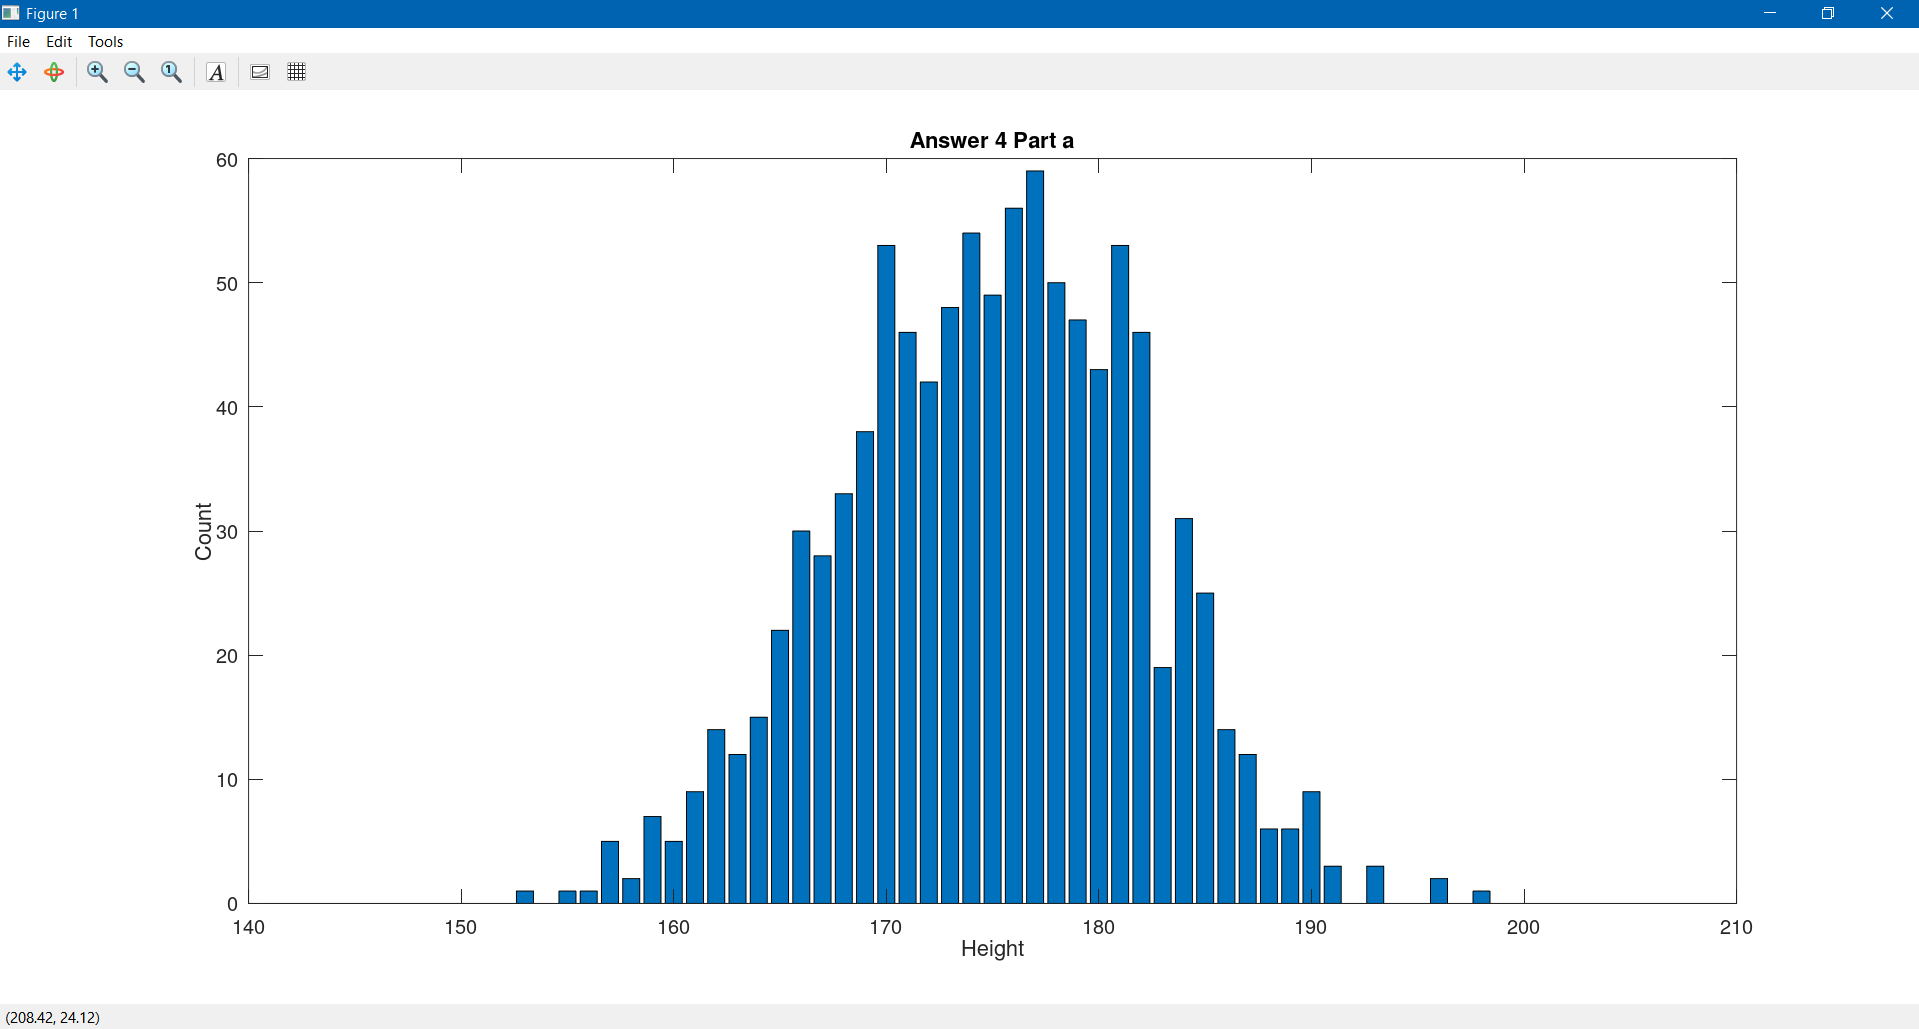
\includegraphics[width=16cm, height=9cm]{a.png} 

\subsubsection*{Comments for a}
In part a we can see that the data is distributed like how it should be in Normal Distribution.
\vspace{0.3cm}\\

\subsection*{b)} 
\begin{Verbatim}[tabsize=4]
data1 = normrnd(175,6,1,1000);
[counts1,bins1] = hist(data1, [150:1:200]);
figure (2);
counts1 = counts1 ./ sum(counts1);
pdf1 = normpdf(bins1,175,6);
pdf1 = pdf1 ./ sum(pdf1);
plot(bins1,pdf1);
title("Answer 4 Part b (sigma=6)");
xlabel("x");
ylabel("f(x)");
set(gca,"fontsize", 20);
set(gca,"ylim", [0 0.1]);
set(gca, "ytick", 0:0.01:0.1);

data2 = normrnd(175,7,1,1000);
[counts2,bins2] = hist(data2, [150:1:200]);
figure (3);
counts2 = counts2 ./ sum(counts2);
pdf2 = normpdf(bins2,175,7);
pdf2 = pdf2 ./ sum(pdf2);
plot(bins2,pdf2);
title("Answer 4 Part b (sigma=7)");
xlabel("x");
ylabel("f(x)");
set(gca,"fontsize", 20);
set(gca,"ylim", [0 0.1]);
set(gca, "ytick", 0:0.01:0.1);

data3 = normrnd(175,8,1,1000);
[counts3,bins3] = hist(data3, [150:1:200]);
figure (4);
counts3 = counts3 ./ sum(counts3);
pdf3 = normpdf(bins3,175,8);
pdf3 = pdf3 ./ sum(pdf3);
plot(bins3,pdf3);
title("Answer 4 Part b (sigma=8)");
xlabel("x");
ylabel("f(x)");
set(gca,"fontsize", 20);
set(gca,"ylim", [0 0.1]);
set(gca, "ytick", 0:0.01:0.1);
\end{Verbatim}

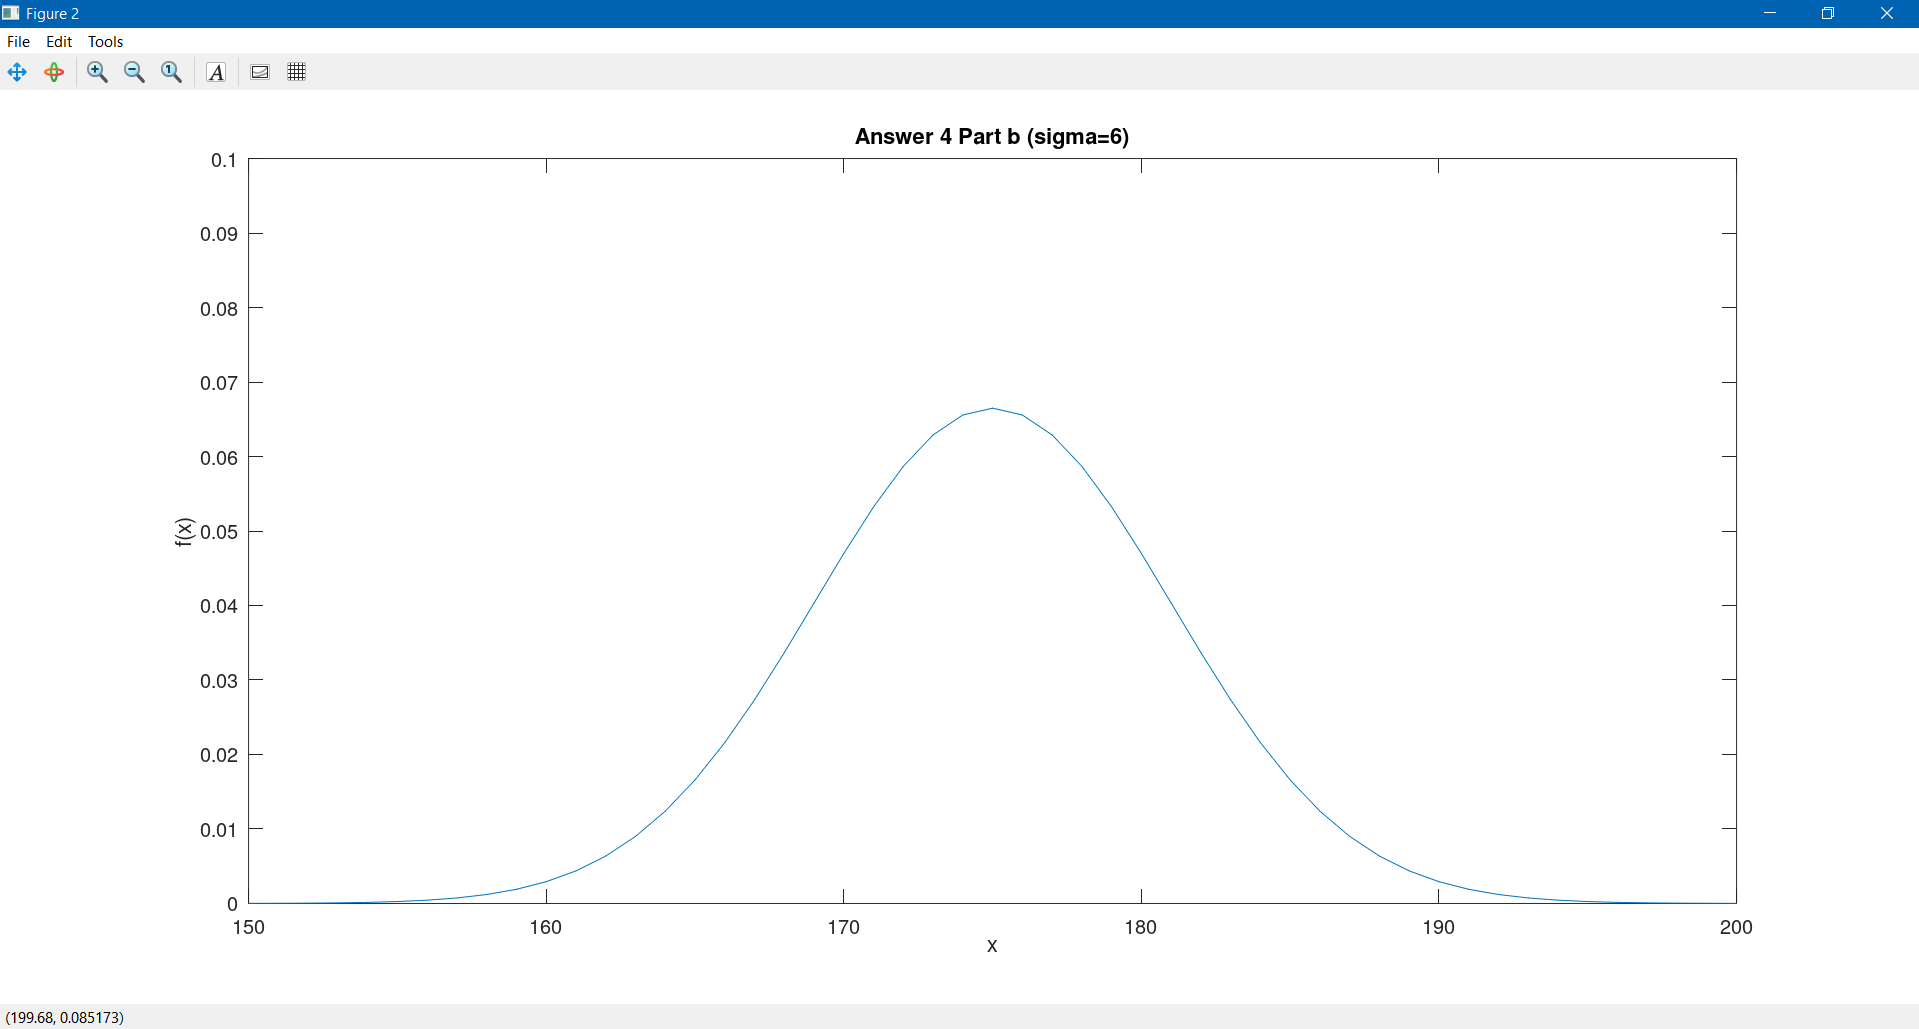
\includegraphics[width=16cm, height=9cm]{b1.png} \\
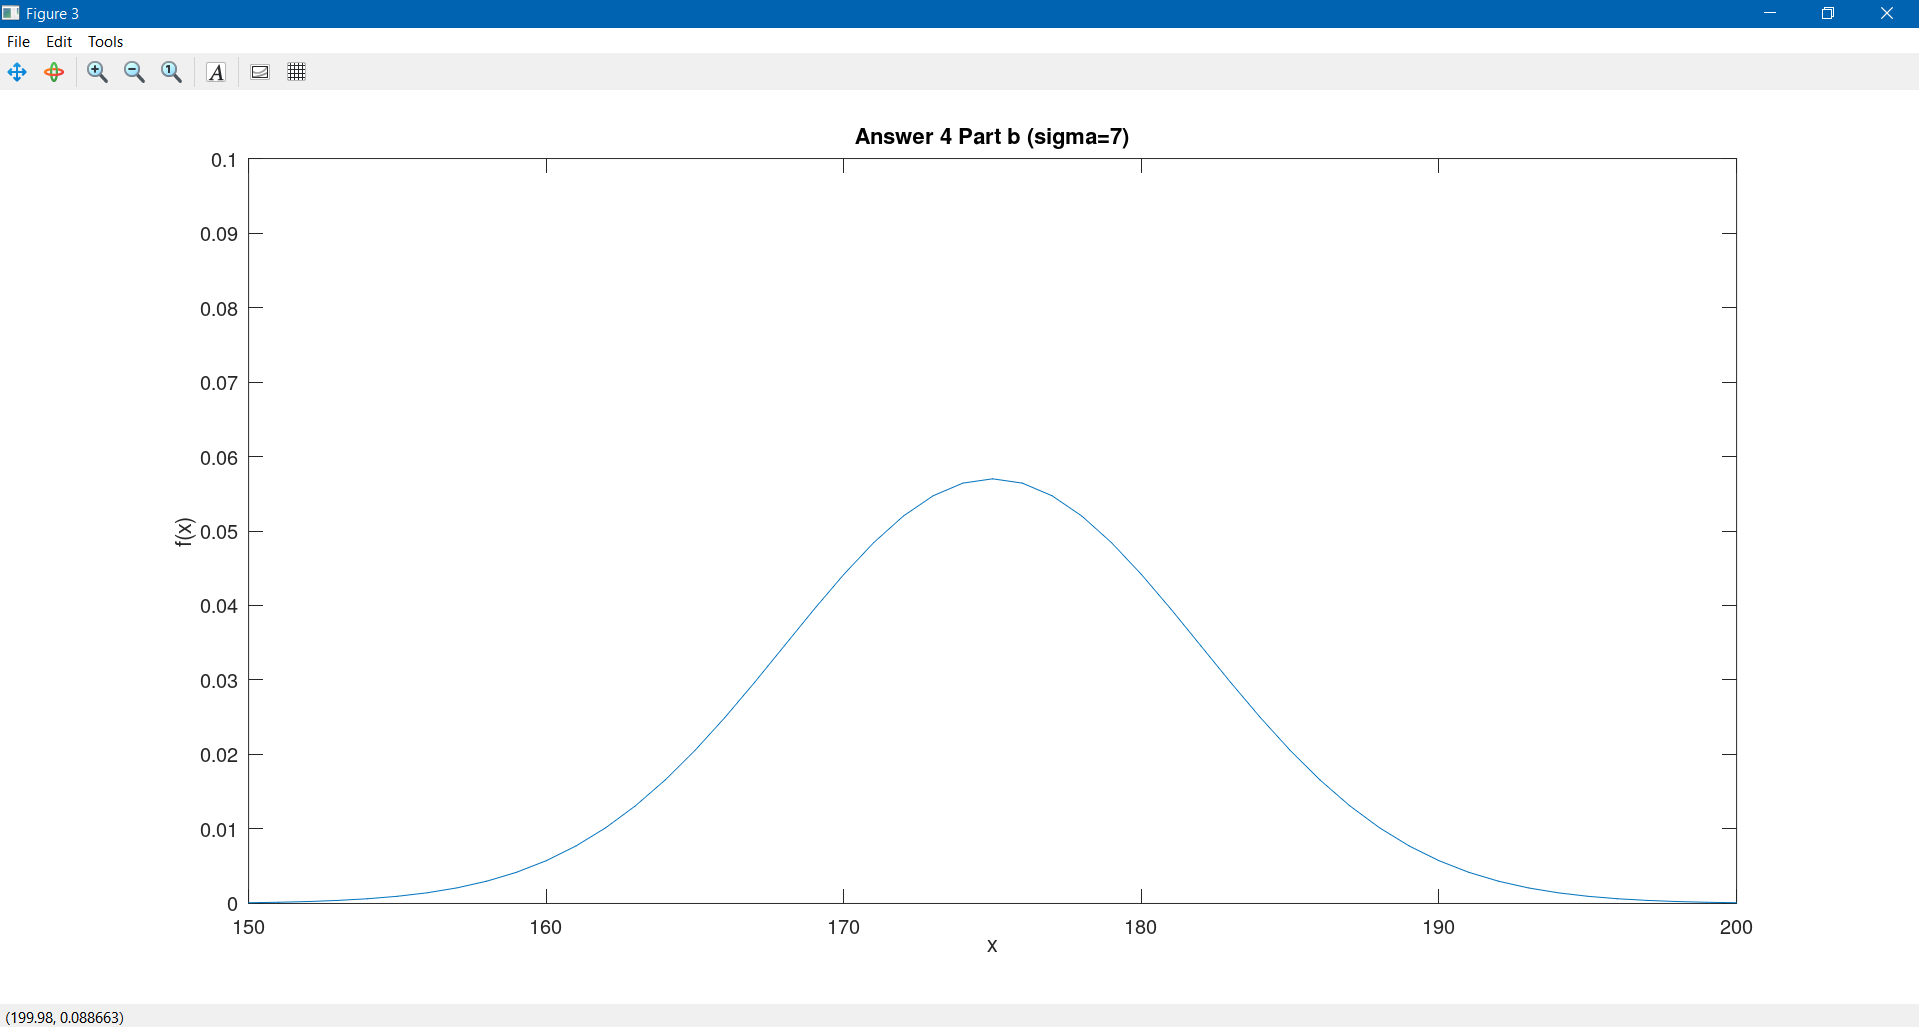
\includegraphics[width=16cm, height=9cm]{b2.png} \\
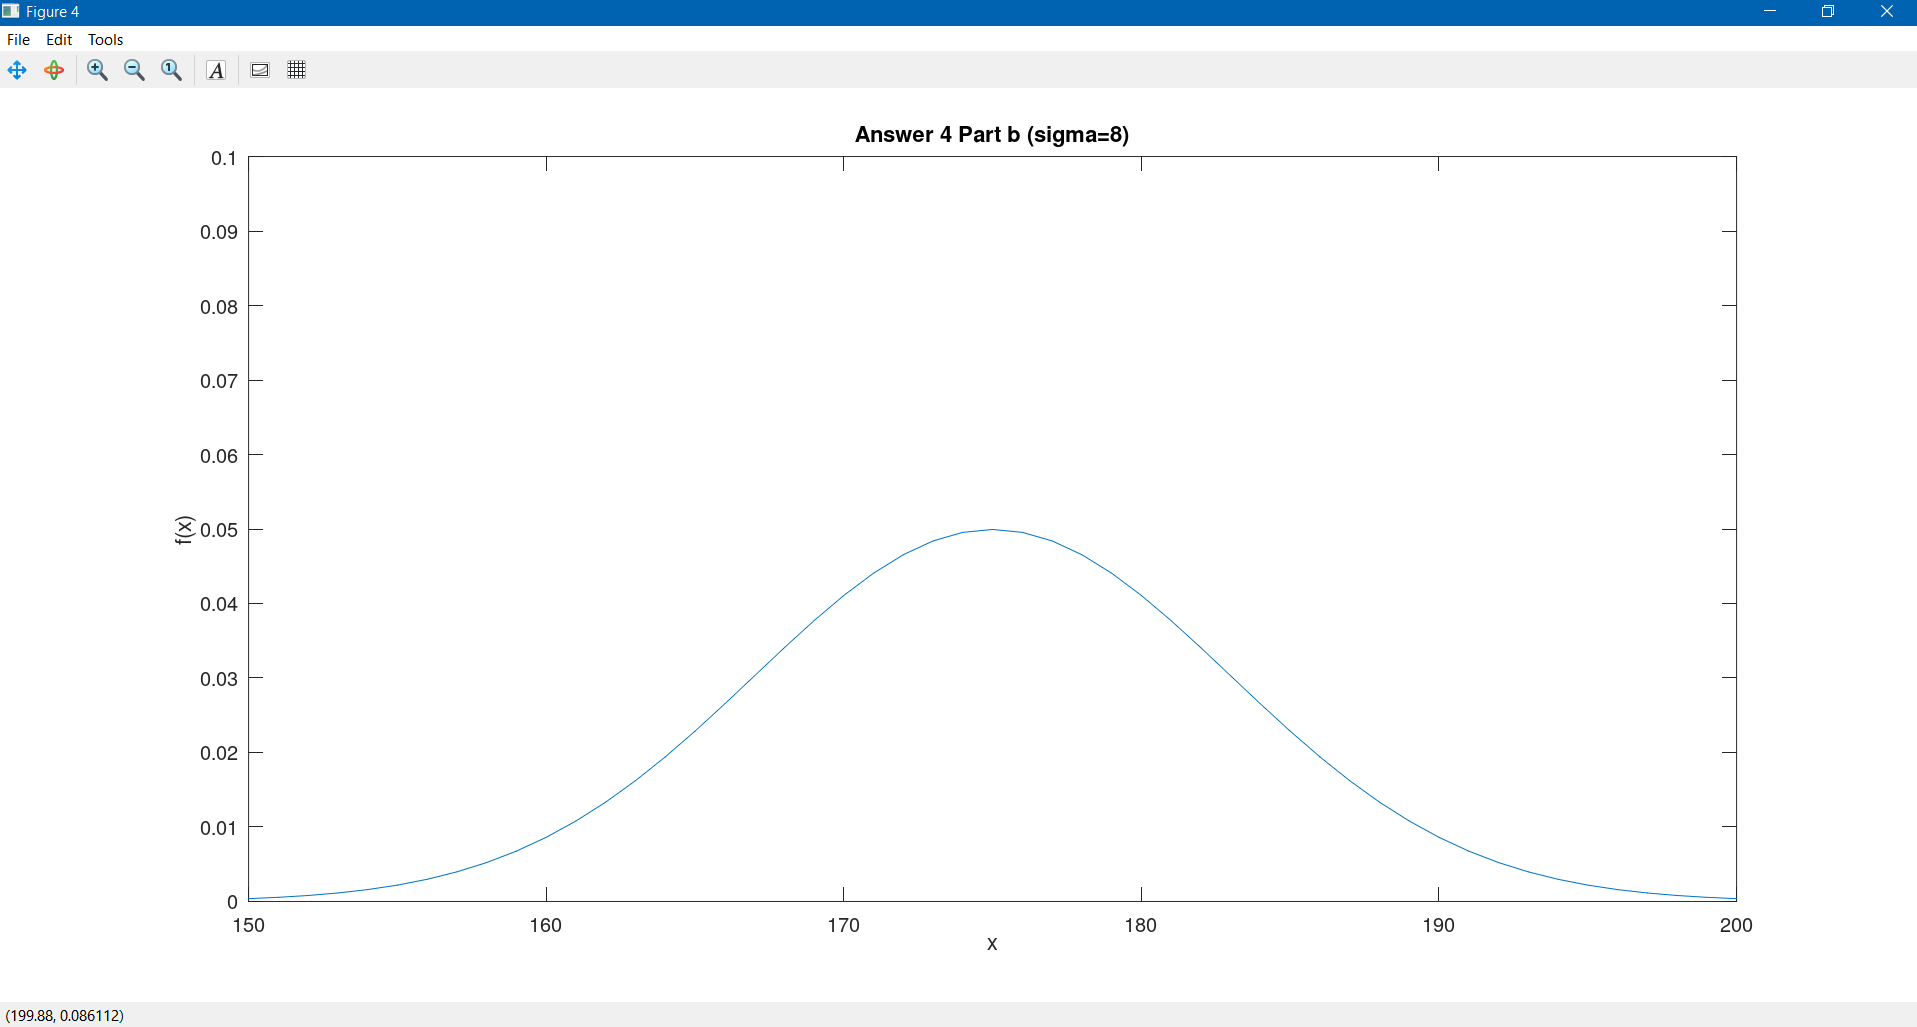
\includegraphics[width=16cm, height=9cm]{b3.png} 

\subsubsection*{Comments for b}
In part b we can see that, when standard deviation is low, data is gathered around the mean and probability is higher around the mean. Whereas, when standard deviation is high, data becomes more distributed to the whole range (between 150 and 200 cm).


\subsection*{c)} 
\begin{Verbatim}[tabsize=4]
perc_array = [];

for j = 1:1000
	data4 = normrnd(175, 7, 1, 1000);
	cnt = 0;
	for i = 1:numel(data4)
		if data4(i) >= 170 && data4(i) <= 180
			cnt++;
		endif
	endfor
	percentage = cnt / numel(data) * 100;
	perc_array = horzcat(perc_array, percentage);
endfor

cnt_45 = 0;
cnt_50 = 0;
cnt_55 = 0;
for i = 1:numel(perc_array)
	if perc_array(i) >= 55
		cnt_45++;
		cnt_50++;
		cnt_55++;
	elseif perc_array(i) >= 50
		cnt_45++;
		cnt_50++;
	elseif perc_array(i) >= 45
		cnt_45++;
	endif
endfor

prob_45 = cnt_45 / numel(perc_array);     # answer of 45%
prob_50 = cnt_50 / numel(perc_array);	 # answer of 50%
prob_55 = cnt_55 / numel(perc_array);     # answer of 55%
\end{Verbatim}

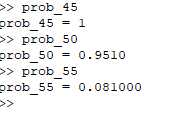
\includegraphics[width=16cm, height=12cm]{c.png} 

\subsubsection*{Comments for c}
In part c we can see that at least 45\% of adults definitely have heights between 170cm and 180cm. Also, at least half of adults having heights between 170cm and 180cm is very likely (95\%). However, at least 55\% of adults having heights between 170cm and 180cm is very unlikely (8\%).


\end{document}